\documentclass{beamer}
\usetheme{Warsaw}

\usepackage[utf8]{inputenc}
\usepackage{fancybox}
\usepackage{multimedia} 
\usepackage{subfig}
\usepackage{amsmath}
\usepackage{hyperref}
\usepackage[all]{xy}
\begin{document}


\title[Stochastik] % (optional, only for long titles)
{Stochastik für Informatiker
\\
\includegraphics[scale=0.5]{img/craps}
}
\subtitle{}
\author[Dr. Johannes Riesterer] % (optional, for multiple authors)
{Dr.  rer. nat. Johannes Riesterer}

\date[KPT 2004] % (optional)
{}

\subject{Stochastik}

\frame{\titlepage}




\begin{frame}
    \frametitle{Statistik - Hypothesentest}
\framesubtitle{}

\begin{block}{Beispiel Entscheidungsfindung - Problemstellung}
Es werden $N= 10.000$ Orangen geliefert. Ist mehr als $5\%$ der Ware verfault, kann der Käufer  die Lieferung an den Verkäufer zurückgehen lassen.
Alle Orangen anschauen ist wegen der Menge allerdings unmöglich.
\end{block}

\begin{block}{Beispiel Entscheidungsfindung - Problemstellung}
Der   Käufer wählt eine Stichprobenmenge  von $n=50$ Orangen  und möchte anhand einer Grenze  $c$ an faulen Orangen innerhalb dieser Stichprobe entscheiden,
ob er die Lieferung zurückgehen lässt oder nicht.  Er wendet also die folgende Entscheidungsregel an:
\begin{center}
höchsten $c$ Orangen  faul $\Rightarrow$ Lieferung akzeptieren \\
mehr als  $c$ Orangen  faul $\Rightarrow$ Lieferung  zurückgehen lassen.
\end{center}
\end{block}



 \end{frame}

\begin{frame}
    \frametitle{Statistik - Hypothesentest}
\framesubtitle{}
\begin{block}{Beispiel Entscheidungsfindung - Problemstellung}
Wie sollte $c$ gewählt werden?
\end{block}


\begin{block}{Beispiel Entscheidungsfindung - Modell}
Man möchte auf der einen Seite, dass die Wahrscheinlichkeit dafür, dass die Lieferung mehr als $5 \%$ faule Orangen enthält nicht erkannt wird, klein ist.
Auf der anderen Seite möchte man auch, dass die Wahrscheinlichkeit für einen  "peinlichen" Fehler, dass die Lieferung zurück geht, obwohl sie weniger als  $5 \%$ faule Orangen enthält, ebenfalls klein ist. 
\end{block}


 \end{frame}

\begin{frame}
    \frametitle{Statistik - Hypothesentest}
\framesubtitle{}
\begin{block}{Beispiel Entscheidungsfindung - Problemstellung}
Wie sollte $c$ gewählt werden?
\end{block}


\begin{block}{Beispiel Entscheidungsfindung - Modell}
Man möchte auf der einen Seite, dass die Wahrscheinlichkeit dafür, dass die Lieferung mehr als $5 \%$ faule Orangen enthält nicht erkannt wird, klein ist.
Auf der anderen Seite möchte man auch, dass die Wahrscheinlichkeit für einen  "peinlichen" Fehler, dass die Lieferung zurück geht, obwohl sie weniger als  $5 \%$ faule Orangen enthält, ebenfalls klein ist. 
\end{block}


 \end{frame}


\begin{frame}
    \frametitle{Statistik - Hypothesentest}
\framesubtitle{}
\begin{block}{Beispiel Entscheidungsfindung - Modell}
Wir modellieren die Anzahl $x$ der faulen Orangen einer Stichprobe $n$ aus der Grundmenge $N$ als "hypergeometrische" Verteilung, wobei die Zahl  $\omega$ der insgesamt faulen  Orangen innerhalb $N$ unbekannt is.
\begin{align*}
P_\omega (x = c)= \frac{\begin{pmatrix} \omega \\ c \end{pmatrix} \cdot  \begin{pmatrix} N - \omega \\ n - c \end{pmatrix}}{\begin{pmatrix} N \\ n \end{pmatrix} }
\end{align*} 
\end{block}


 \end{frame}


\begin{frame}
    \frametitle{Statistik - Hypothesentest}
\framesubtitle{}
\begin{block}{Beispiel Entscheidungsfindung - Modell}
Ist $x$ die Anzahl der faulen Orangen in einer Stichprobe $n = 50$, so lauten unsere vorigen Überlegung mit Hilfe des Modells: Wähle Schranke $c$ für faule Orangen in Stichprobe so,  dass für $\alpha = 0.025$
\begin{align*}
& P_\omega( x >c) < \alpha  \text{ für } \omega < 500 (= 5 \% \text{ von } N = 10.000) \\
& P_\omega( x >c) \text{ möglichst groß für } \omega > 500\\
\end{align*}
gilt.
\end{block}

\begin{block}{Beispiel Entscheidungsfindung - Modell}
Die genaue Bestimmung von $c$ ist auf den ersten Blick nicht so einfach. Wir werden das Problem auf eine einfachere Situation, einen sogenannten Neyman-Pearson-Test, zurückführen. 
\end{block}


 \end{frame}


\begin{frame}
    \frametitle{Statistik - Hypothesentest}
\framesubtitle{}
\begin{block}{Test}
Sei   $(\mathcal{X}, \mathcal{F}, P_\rho :  \rho \in \Theta)$ ein statistisches Modell und $ \Theta =  \Theta_0 \cup  \Theta_1$ eine Zerlegung.  Wir nennen $H_0 : \rho \in \Theta_0$ die Nullhypothese und  $H_1 : \rho \in \Theta_1$ die Alternative 
und eine Statistik $\varphi: \mathcal{X} \to [0,1]$ einen Test von $H_0$ gegen $H_1$. $\{ x \in \mathcal{X}  : \varphi(x) = 1\}$ heißt Ablehnungsbereich und  $\{ x \in \mathcal{X}  : \varphi(x) = 0\}$   Annahmebereich des Tests $\varphi$
\end{block}
\begin{block}{Gütefunktion}
Die Funktion $G_{\varphi}: \Theta \to [0,1], G_{\varphi}(\rho) = \mathbb{E}_{\rho}(\varphi)$ heißt Gütefunktion des Tests.
\end{block}
 \end{frame}

\begin{frame}
    \frametitle{Statistik - Hypothesentest}
\framesubtitle{}
\begin{block}{Signifikanz-Niveau}
Die im ungünstigen Fall vorliegende Wahrscheinlichkeit für einen Fehler erster Art ist $\sup_{\rho \in \Theta_0} \mathbb{E}_{\rho}(\varphi)$. Sie heißt Niveau von $\varphi$.  Ein Test hat das (Signifikanz-)Niveau $\alpha$, falls  $\sup_{\rho \in \Theta_0} \mathbb{E}(\varphi) \leq \alpha$.
\end{block}
\begin{block}{Macht}
Für $\rho \in \Theta_1$ heißt  $ G_{\varphi}(\rho)$ die Macht von $\varphi$ bei $\rho$. Sie ist die Wahrscheinlichkeit, mit der die Alternative erkannt wird, wenn sie vorliegt und $\beta_{\varphi}(\rho) = 1 - G_{\varphi}(\rho)$ ist die Wahrscheinlichkeit für einen Fehler zweiter Art, nämlich dass das Vorliegen der Alternative nicht erkannt wird und deshalb die Nullhypothese fälschlich akzeptiert wird.
\end{block}
 \end{frame}

\begin{frame}
    \frametitle{Statistik - Hypothesentest}
\framesubtitle{}

\begin{figure}[htp]
      \centering
Gütefunktion eines Binomialtests mit $n = 30$. Für alle Werte von $p$ aus der Nullhypothese $H0: p \leq 0,2$ liegt $G(p)$ unter dem Signifikanzniveau $\alpha = 5 \%$.

      \centering
    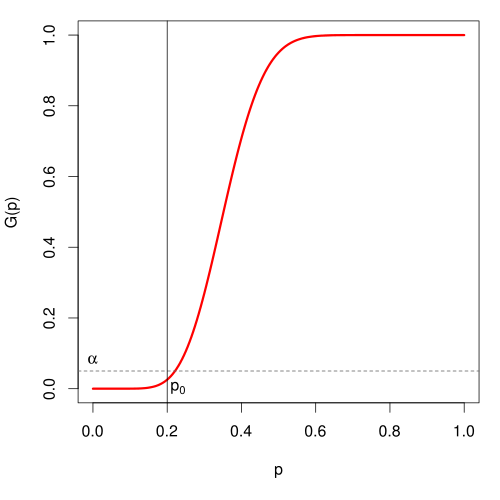
\includegraphics[width=0.5\textwidth]{img/Power_function_binomial_test}
\caption{Quelle: Wikipedia}
\end{figure}

 \end{frame}



\begin{frame}
    \frametitle{Statistik - Hypothesentest}
\framesubtitle{}
\begin{block}{Gütefunktion}
Ein Test $\varphi$ von $H_0$ gegen $H_1$ heißt bester Test zum Niveau $\alpha$, falls für jeden anderen Test $\psi$ zum 
 Niveau $\alpha$ gilt:
\begin{align*}
G_{\varphi}(\rho) \geq G_{\psi}(\rho) \text{ für alle } \rho \in \Theta_1
\end{align*}
Er erkennt also von allen Tests am Besten die Alternative unter Einhaltung  des Signifikanz-Niveau für den ungünstigen Fehler.
\end{block}

 \end{frame}


\begin{frame}
    \frametitle{Statistik - Hypothesentest}
\framesubtitle{}
\begin{block}{Neyman-Pearson-Test}
Sei   $(\mathcal{X}, \mathcal{F}, P_0, P_1)$ ein statistisches Modell mit $\Theta = \{ 0,1\}$ und Dichten $p_0$ und $p_1$ von $P_0$ und $P_1$ und dem Likelyhood-Quotienten
 \begin{align*}
 R(X) = \begin{cases} \frac{p_1(x)}{p_0(x)} \text{ falls } p_0(x) > 0 \\ \infty  \text{ falls } p_0(x) = 0 \end{cases}
\end{align*}. 
Der Test 
\begin{align*}
 \varphi(x) = \begin{cases} 1 \text{ falls } R(x) > c \\ 0  \text{ falls } R(x) < c \end{cases}
\end{align*}
heißt Neyman-Pearson-Test zum Schwellwert $c$. $R(x) = c$ kann hierbei beliebig gesetzt werden.
\end{block}

 \end{frame}


\begin{frame}
    \frametitle{Statistik - Hypothesentest}
\framesubtitle{}
\begin{block}{Neyman-Pearson Lemma}
Sei   $(\mathcal{X}, \mathcal{F}, P_0, P_1)$ ein statistisches Modell. Dann gilt:
\begin{enumerate}
\item Zu gegebenen $\alpha$ gibt es einen Neyman-Pearson-Test  $\varphi$ mit Niveau $\mathbb{E}_0(\varphi) = \alpha$.
\item Dieser Test ist ein bester Test zum Niveau $\alpha$. Jeder Beste Test   zum Niveau $\alpha$ ist nicht unterscheidbar von diesem.
\end{enumerate}
\end{block}

 \end{frame}


\begin{frame}
    \frametitle{Statistik - Hypothesentest}
\framesubtitle{}
\begin{block}{Quantil und Fraktil}
Sei $Q$ ein Wahrscheinlichkeitsmass auf $(\mathbb{R}, \mathcal{B}(\mathbb{R}) )$ und $0 < \alpha <1$. Dann heißt jede Zahl $q \in \mathbb{R}$ mit $Q((-\infty, q ]) \geq \alpha$ und  $Q((q, \infty )) \geq 1- \alpha$  ein $\alpha$-Quantil von $Q$.
\begin {itemize}
\item $\alpha = \frac{1}{2}$ heißt Media.
\item $\alpha = \frac{1}{4}$ und  $\alpha = \frac{3}{4}$ heißen Quartile.
\item Ein $(1-\alpha)$-Quantil heißt $\alpha$-Fraktil. 
\end{itemize}
\end{block}

\begin{figure}[htp]
      \centering
    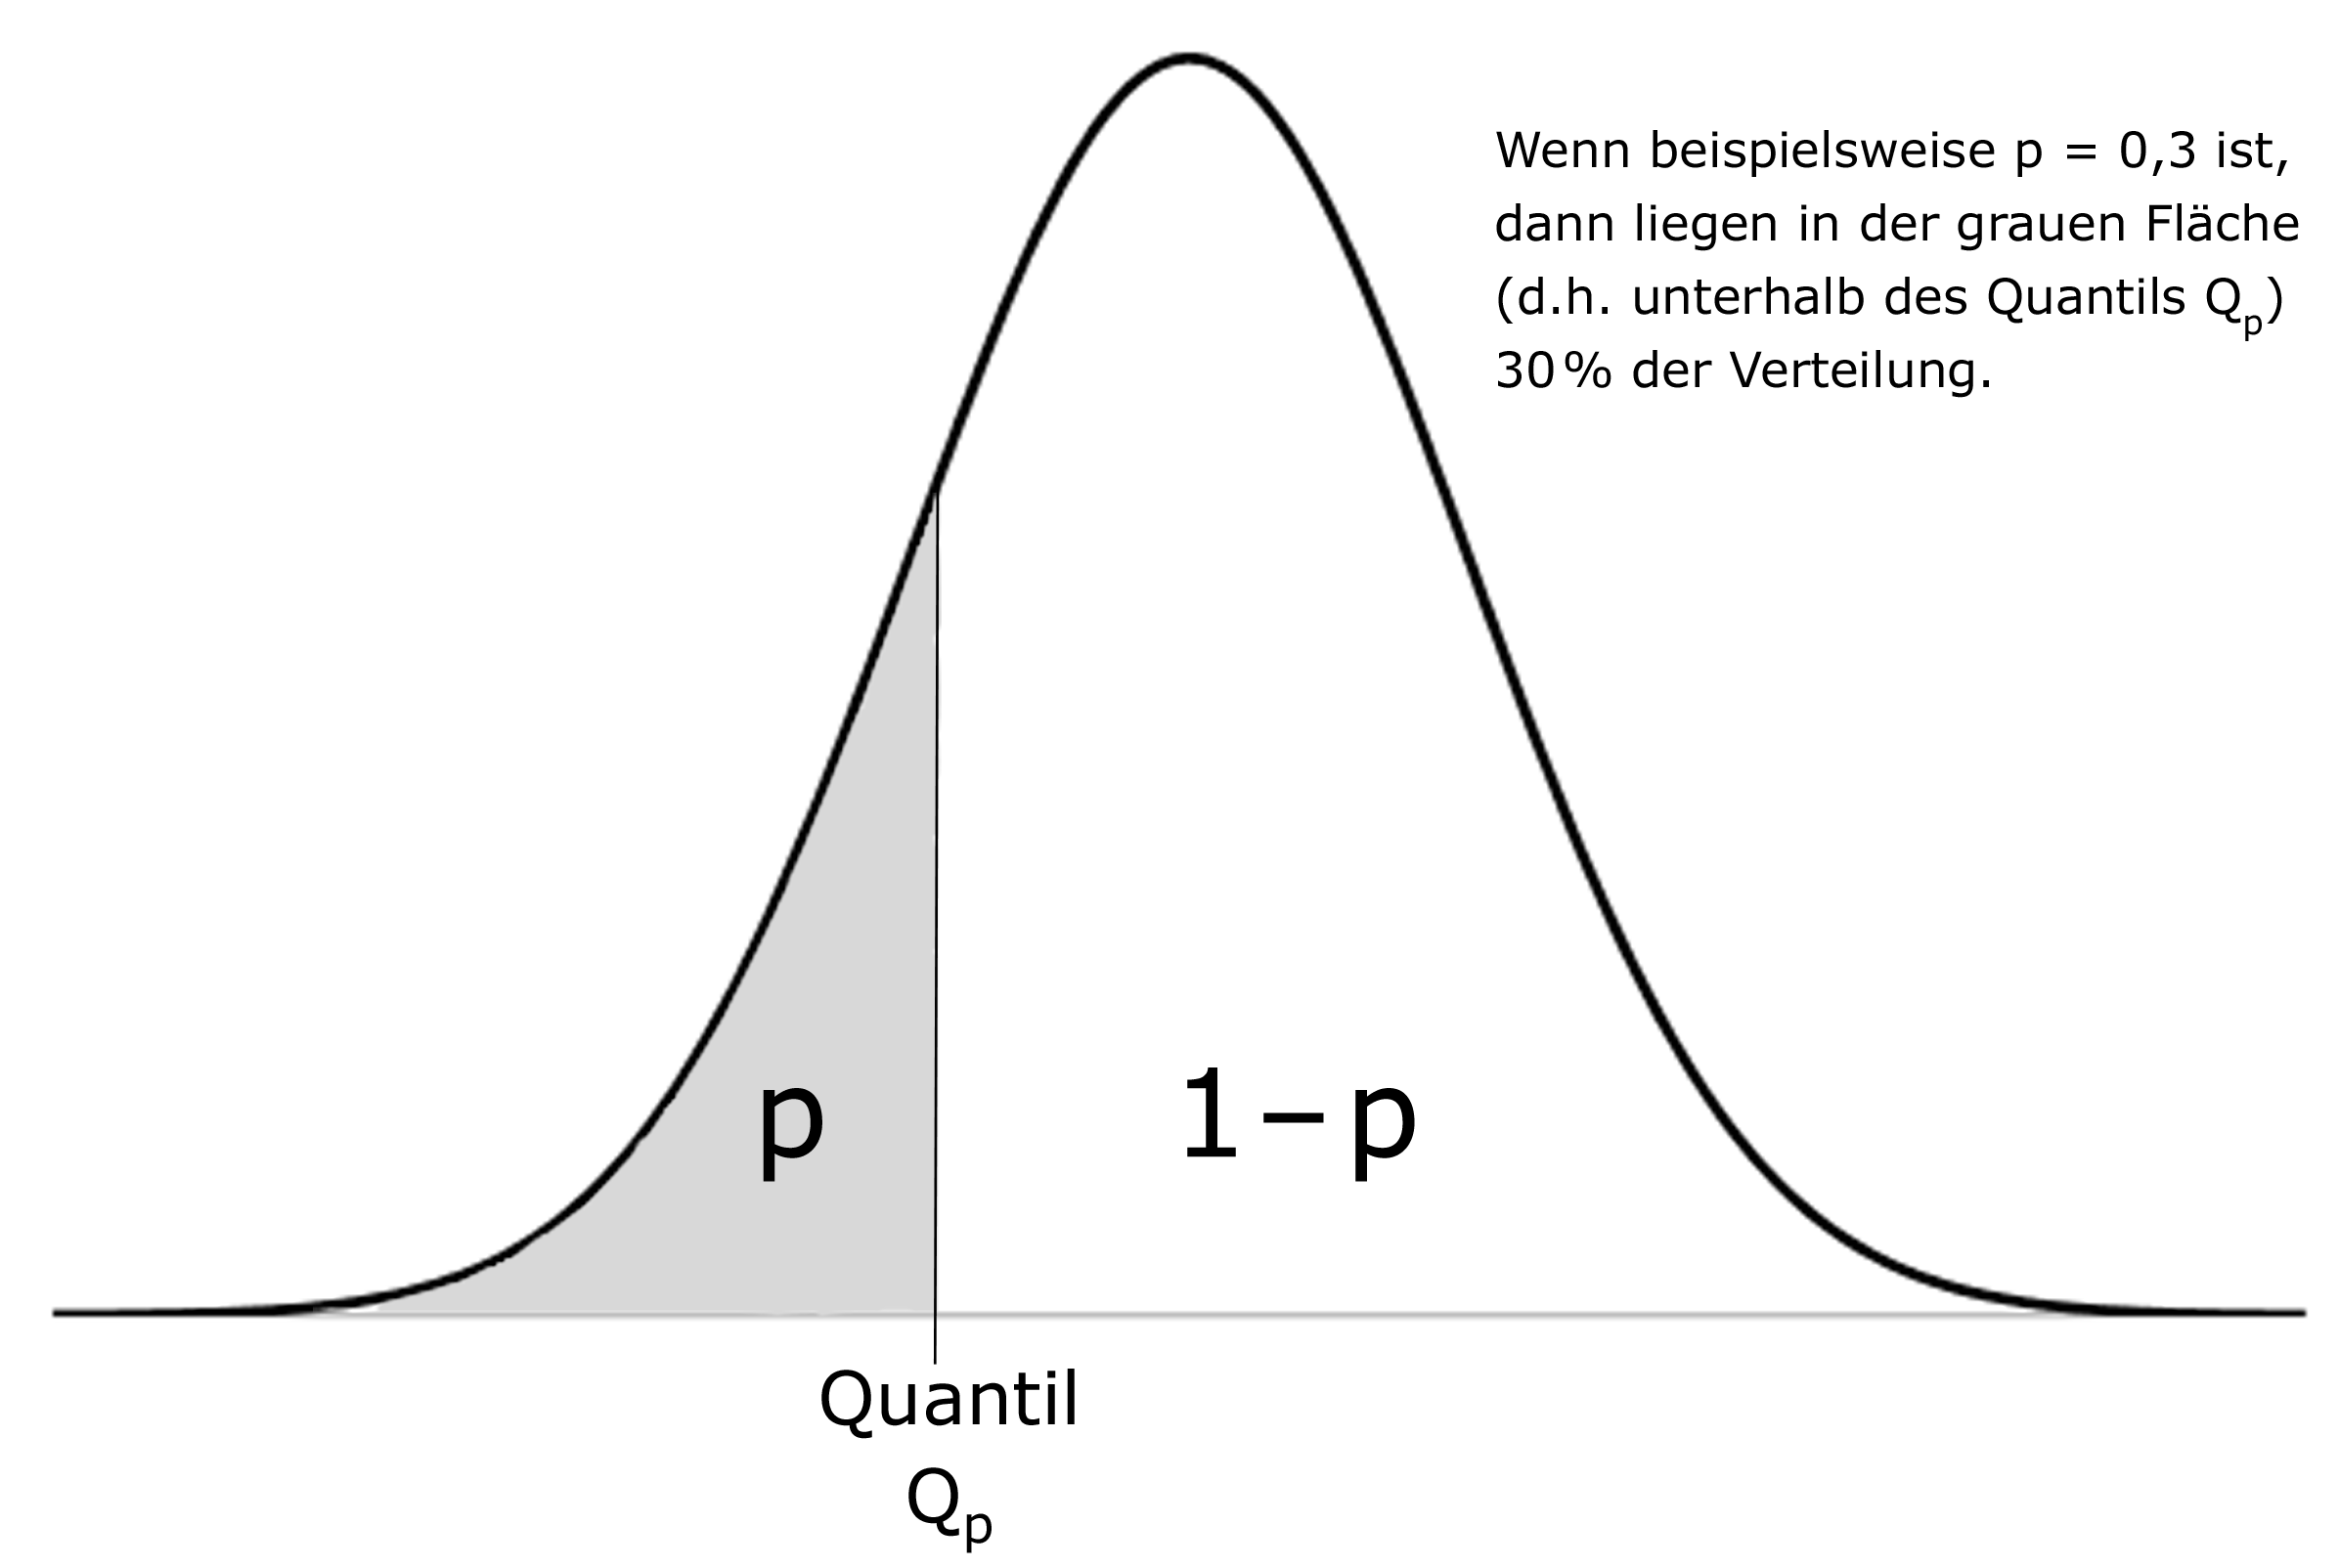
\includegraphics[width=0.45\textwidth]{img/Quantil}
      \caption{Quelle: Wikipedia}
\end{figure}

 \end{frame}


\begin{frame}
    \frametitle{Statistik - Hypothesentest}
\framesubtitle{}
\begin{block}{Beweis}
Sei $c$ ein $\alpha$-Fraktil des Wahrscheinlichkeitsmasses $P_0 \circ R^{-1}$. Definitionsgemäß gilt also $P_0(R \geq c) \geq \alpha$ und $P_0 (R > c) = 1 - \underbrace{P_0(R \leq \alpha)}_{\geq 1 - \alpha} \leq \alpha$. Folglich gilt
$\alpha - P_0(R >c) \leq P_0(R \geq c) - P_0(R > c) = P_0(R = c) $. \\
Ist $ P_0(R = c)  = 0$ so ist $ P_0(R >c) = \alpha$ und $\varphi = 1_{R > c}$ ein Neyman-Pearson-Test mit $\mathbb{E}_0(\varphi) = \alpha$. 
\\ Ist $ P_0(R = c) > 0$, so ist
\begin{align*}
\gamma := \frac{\alpha - P_0(R > c)}{ P_0(R=c)} \in [0,1]
\end{align*}
\end{block}

 \end{frame}


\begin{frame}
    \frametitle{Statistik - Hypothesentest}
\framesubtitle{}
\begin{block}{Beweis}
Damit ist 
\begin{align*}
 \varphi(x) = \begin{cases} 1 \text{ falls } R(x) > c \\  \gamma  \text{ falls } R(x) = c \\ 0 \text{ falls } R(x) < c  \end{cases}
\end{align*}
ein Neyman-Pearson-Test mit $\mathbb{E}_0(\varphi) = P_0(R > c) + \gamma P_0(R=c) = \alpha$.
\end{block}

 \end{frame}



\begin{frame}
    \frametitle{Statistik - Hypothesentest}
\framesubtitle{}
\begin{block}{Beweis}
Sei $\varphi$ ein Neyman-Pearson-Test  mit $\mathbb{E}_0(\varphi) = \alpha$ und Schwellenwert $c$ sowie $\psi$ ein beliebiger Test zum Niveau $\alpha$. Ist $\varphi(x) > \psi(x)$, so ist $\varphi(x) > 0$, also $R(x) \geq c$ und daher $p_1(x) \geq c p_0(x)$. Ist $\varphi(x) < \psi(x)$ ist $\varphi(x) <1$ und also $p_1(x) \leq c p_0(x)$. Es gilt also immer
\begin{align*}
f_1(x) := (\varphi(x) - \psi(x))p_1(x) \geq c ( \varphi(x) - \psi(x))p_0(x) ) := c \; f_0(x)
\end{align*}
Integration (bzw. Summation im diskreten Fall) liefert
\begin{align*}
\mathbb{E}_1(\varphi) - \mathbb{E}_1(\psi) = \int_{\mathcal{X}} f_1(x) dx \geq c   \int_{\mathcal{X}} f_0(x) dx = c(\alpha -  \mathbb{E}_0(\psi)  ) \geq 0
\end{align*}
und damit ist $\varphi$ ein bester Test.
\end{block}

 \end{frame}

\begin{frame}
    \frametitle{Statistik - Hypothesentest}
\framesubtitle{}
\begin{block}{Beweis}
Ist  $\psi$ ein beliebiger bester Test, so gilt in obigen Ungleichungen überall Gleichheit und damit $\varphi = \psi$ fast überall (bis auf Nullmenge). Damit ist auch $\psi$ ein Neumann-Pearson-Test.
\end{block}

 \end{frame}


\begin{frame}
    \frametitle{Statistik - Hypothesentest}
\framesubtitle{}


\begin{block}{Beispiel Entscheidungsfindung - Lösung}
Im Beispiel der Orangenlieferung  setzen wir $\Theta_0 = \{ 0, \cdots \rho_0 \}$ und $\Theta_1 = \{\rho_0 +1 , \cdots N \}$ mit $\rho_0 = 500$ und betrachten den Test
\begin{align*}
 \varphi(x) = \begin{cases} 1 \text{ falls } A(x) > c \\  \gamma  \text{ falls } A(x) = c \\ 0 \text{ falls }A(x) < c  \end{cases}
\end{align*}
zur Hypothese $H_0: \rho \in \Theta_0$ und der Alternative $H_1: \rho \in \Theta_1$. Hierbei ist $A$ die Funktion, die die Anzahl an faulen Orangen zählt. 
Wir möchten $c$ nach Möglichkeit  so bestimmen, dass der Test $\varphi$ optimal ist. Wir wählen  $c$ als $\alpha$-Fraktil von $P_{\rho_0}$.  $\gamma$ ergibt sich dann aus
\begin{align*}
G_{\varphi}(\rho_0) = P_{\rho_0} (\{ c+1, \cdots, n \}) + \gamma  P_{\rho_0}(\{ c\}) = \alpha 
\end{align*}
\end{block}

 \end{frame}


\begin{frame}
    \frametitle{Statistik - Hypothesentest}
\framesubtitle{}

\begin{block}{Beispiel Entscheidungsfindung - Lösung}
Für $\rho' > \rho$ ist der Likelyhood-Quotient  $R_{\rho' : \rho} (x):= \frac{p_{\rho' (x)}}{p_{\rho}(x)}$ monoton wachsend in $x$, da
\begin{align*}
R_{\rho' : \rho} (x)= \prod_{k = \rho}^{\rho'-1} \frac{(k+1)(N -k -n +x)}{(N-k) (k+1 -x)}
\end{align*}
Setzen wir  $\bar{c}:= R_{\rho' : \rho} (c)$, dann gilt wegen der Monotonie: Ist $R_{\rho' : \rho} (x) > \bar{c}$ so ist $ x >c$ und daher $\varphi(x) = 1$. Im Fall  $R_{\rho' : \rho} (x) < \bar{c}$ ergibt sich ebenso $\varphi(x) = 0$. $\varphi$ is also ein Neyman-Pearson-Test der Nullhypothese $\{\rho\}$ gegen $\{\rho' \}$. Für $\rho = \rho_0$ und beliebiges $\rho' \in \Theta_1$ ist $\varphi$ damit ein bester Test für die Hypothese $H_0: \rho = \rho_0$ gegen  $H_1: \rho \in  \Theta_1$ zum Niveau $\alpha$.

\end{block}

 \end{frame}



\begin{frame}
    \frametitle{Statistik - Hypothesentest}
\framesubtitle{}

\begin{block}{Beispiel Entscheidungsfindung - Lösung}
Wir müssen also noch zeigen, dass es auch ein bester Test für alle $\rho \in \Theta_0$ zum Niveau $\alpha$ ist. 
Da  $G_{\varphi} (\rho) \leq \alpha$ für alle $\rho \in \Theta_0$  gelten muss und nach Konstruktion und $G_{\varphi} (\rho_0) = \alpha$, reicht zu zeigen, dass die Gütefunktion  $G_{\varphi}$ monoton wachsend ist. Für $\rho < \rho'$ ist $\varphi$ ein bester Test zum Niveau $\beta = G_{\varphi} (\rho)$ und damit ist er besser als der konstante Test  $\psi = \beta$. Es folgt  
$G_{\varphi} (\rho') \geq G_{\psi} (\rho') = \beta = G_{\varphi} (\rho) $ und damit ist die Gütefunktion  wachsend.
\end{block}

 \end{frame}



\begin{frame}
    \frametitle{Statistik - Hypothesentest}
\framesubtitle{}

\begin{block}{Beispiel Entscheidungsfindung - Lösung}
Es ergibt sich $c = 6$ und $\gamma = 0.52$.
\end{block}

 \end{frame}



\begin{frame}
    \frametitle{Statistik - Hypothesentest}
\framesubtitle{}

\begin{block}{Einseitiger Test mit monotonem Lieklyhood-Quotienten}
Sei   $(\mathcal{X}, \mathcal{F}, P_\rho :  \rho \in \Theta \subset \mathbb{R})$ ein statistisches Modell mit Dichte $p_{\rho}$ von $P_\rho$ und wachsendem  Likelyhood-Quotient  $R_{\rho' : \rho} (x):= \frac{p_{\rho' (x)}}{p_{\rho}(x)}$ bezüglich einer Statistik  $T$ (Dies bedeutet: $R_{\rho' : \rho} (x) > f_{\rho', \rho} \circ T$ mit einer wachsenden Funktion $f_{\rho', \rho}$). Dann ist für einen  Schwellenwert $\rho_0 \in \Theta$ und ein Niveau $0 <\alpha < 1$ der Test 
\begin{align*}
 \varphi(x) = \begin{cases} 1 \text{ falls } T(x) > c \\  \gamma  \text{ falls } T(x) = c \\ 0 \text{ falls } T(x) < c  \end{cases}
\end{align*}
ein optimaler Test für die Nullhypothese $H_0 : \rho \leq \rho_0$ gegen die Alternative  $H_1 : \rho > \rho_0$. 
$c$ und $\gamma$ lassen sich aus der Beziehung
\begin{align}
G_\varphi(\rho_0) = \alpha  \Leftrightarrow P_{\rho_0}(T  > c) + \gamma P_{\rho_0}(T = c) = \alpha
\end{align}
 bestimmen.
\end{block}



 \end{frame}



\begin{frame}
    \frametitle{Statistik - Hypothesentest}
\framesubtitle{}

\begin{block}{Beweis}
Analog zu  Beispiel mit Orangenlieferung!
\end{block}

 \end{frame}

\begin{frame}
    \frametitle{Statistik - Hypothesentest}
\framesubtitle{}

\begin{block}{Konkrete Bestimmung von $c$: Fall  $P_{\rho_0}(T  = c) = 0$ (kontinuierlicher Fall)}

Wähle $\rho_0 = \max_{\rho} \rho \in \Theta_0$. Wegen  Gleichung $(1)$   muss dann $P_{\rho_0}(T  > c) \leq \alpha$ gelten.  Dies ist gleichbedeutend mit der Bedingung $P_{\rho_0}(T  \leq c)  \geq 1 - \alpha$. Damit ist $c$ gerade das $(1-\alpha)$-Quantil (bzw. das $\alpha$-Fraktil) der Verteilung des Schätzers $P_{T_{\rho_0}}$ bei fester Wahl des Parameters $\rho = \rho_0$. Kennt man diese Verteilung, kann man das  $(1-\alpha)$-Quantil und damit $c$ in entsprechenden Tabellen einfach nachschlagen.  
\end{block}


 \end{frame}
\begin{frame}
    \frametitle{Statistik - Hypothesentest}
\framesubtitle{}

\begin{block}{Konkrete Bestimmung von $c$: Fall  $P_{\rho_0}(T  = c) \neq 0$ (diskreter Fall)}
Wähle $\rho_0 = \max_{\rho} \rho \in \Theta_0$. Da $\gamma \in [0,1]$ muss  für $\gamma =1$ wegen Gleichung $(1)$  $P_{\rho_0}(T  \geq c)  \leq \alpha$ gelten.  Dies ist gleichbedeutend mit der Bedingung $1 - P_{\rho_0}(T  < c)  \leq \alpha$. Wir müssen das kleinste $c$ finden, so dass $1 - P_{\rho_0}(T  \leq c -1)  \leq \alpha$ ist.  Dies ist gleichbedeutend mit  $P_{\rho_0}(T  \leq c -1)  \geq 1- \alpha$. Wir können damit $c-1$ mit Hilfe einer Verteilungstabelle oder als $(1-\alpha)$-Quantil in einer Quantils-Tabelle  der Verteilung des Schätzers $P_{T_{\rho_0}}$ bei fester Wahl des Parameters $\rho = \rho_0$ ermitteln.

\end{block}


 \end{frame}





\end{document}
